\chapter{Dictionary Word Sets} \label{dictionary_sets}

\begin{figure}[h]
	\centering
	%\vspace{150pt}
	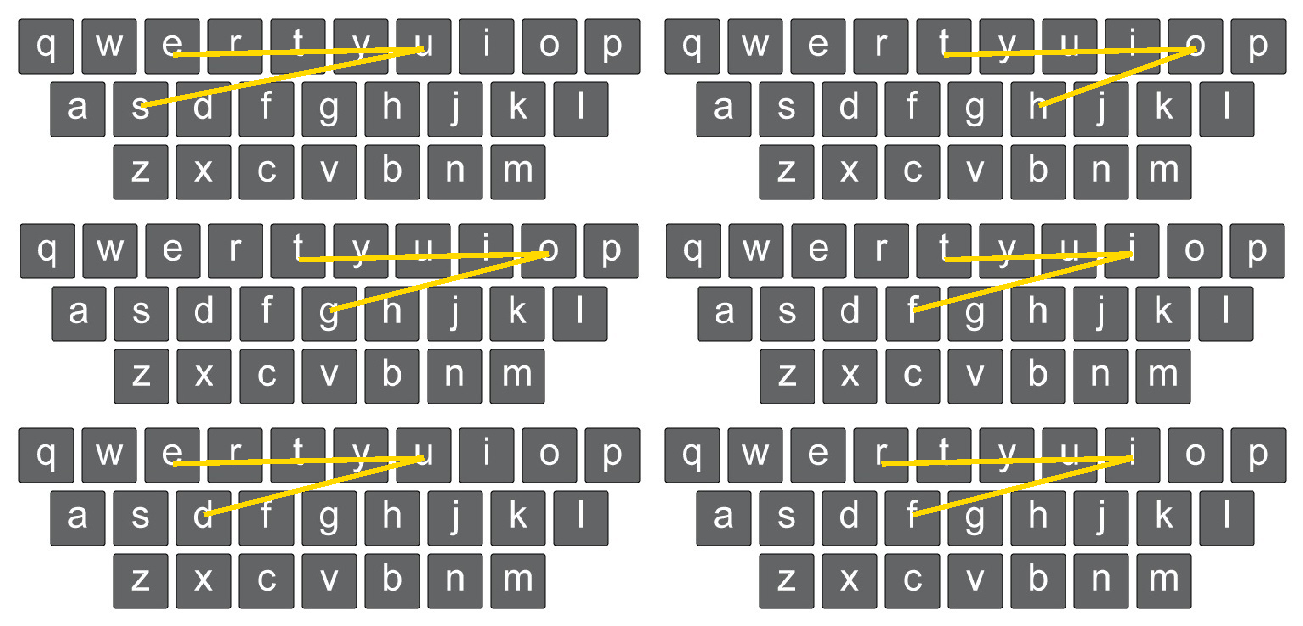
\includegraphics[width=5in]{Figures/fig_words_1}
	\caption[Word Set 1]{The similar gesture-shapes of the word set: `sue', `hot', `got', `fit', `due', `fir'. These gesture-shapes were generated by minimizing dissimilarity using the custom dissimilarity algorithm in Section~\ref{gesture_shape_dissimilarity}.}
	\label{fig_words_1}
\end{figure}

\clearpage

\begin{figure}[t]
	\centering
	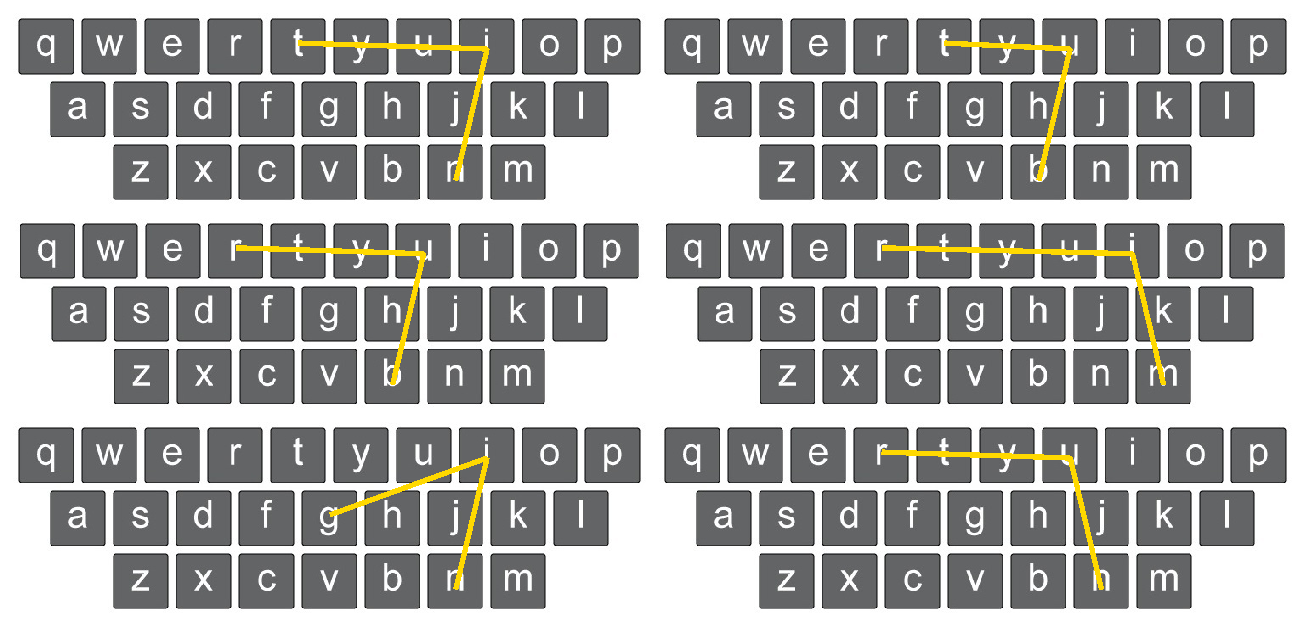
\includegraphics[width=5in]{Figures/fig_words_2}
	\caption[Word Set 2]{The similar gesture-shapes of the word set: `tin', `tub', `rub', `rim', `gin', `run'. These gesture-shapes were generated by minimizing dissimilarity using the custom dissimilarity algorithm in Section~\ref{gesture_shape_dissimilarity}.}
	\label{fig_words_2}
\end{figure}

\begin{figure}[b]
	\centering
	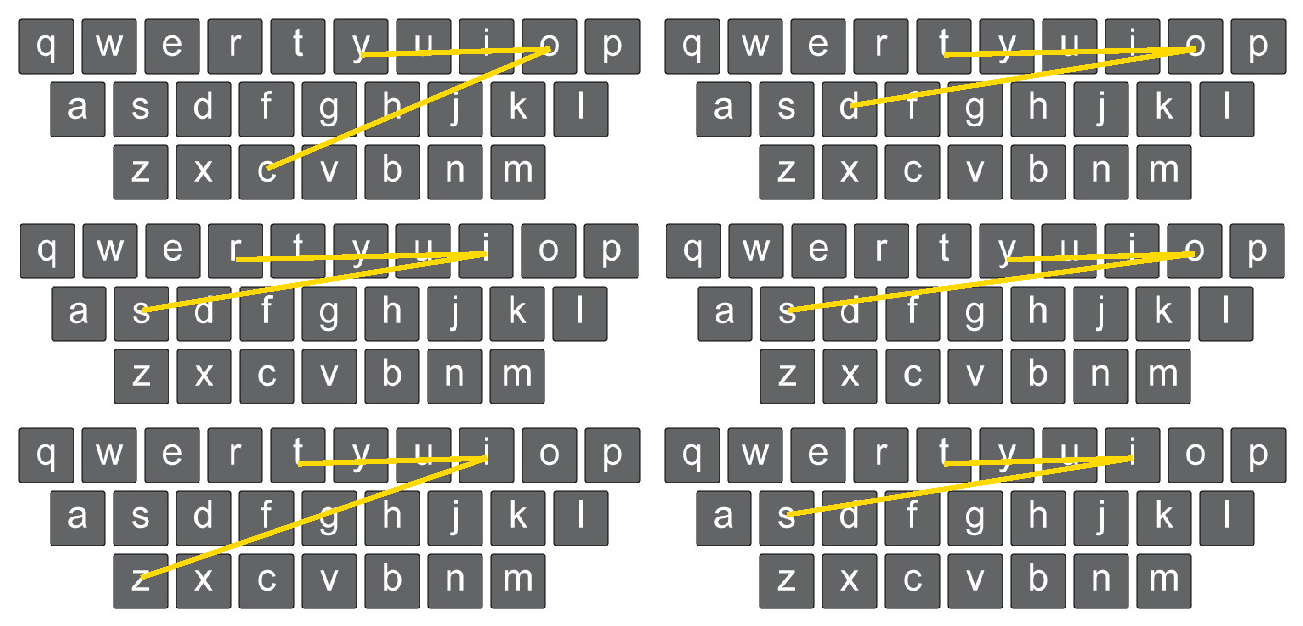
\includegraphics[width=5in]{Figures/fig_words_3}
	\caption[Word Set 3]{The similar gesture-shapes of the word set: `coy', `dot', `sir', `soy', `zit', `sit'. These gesture-shapes were generated by minimizing dissimilarity using the custom dissimilarity algorithm in Section~\ref{gesture_shape_dissimilarity}.}
	\label{fig_words_3}
\end{figure}

\clearpage

\begin{figure}[t]
	\centering
	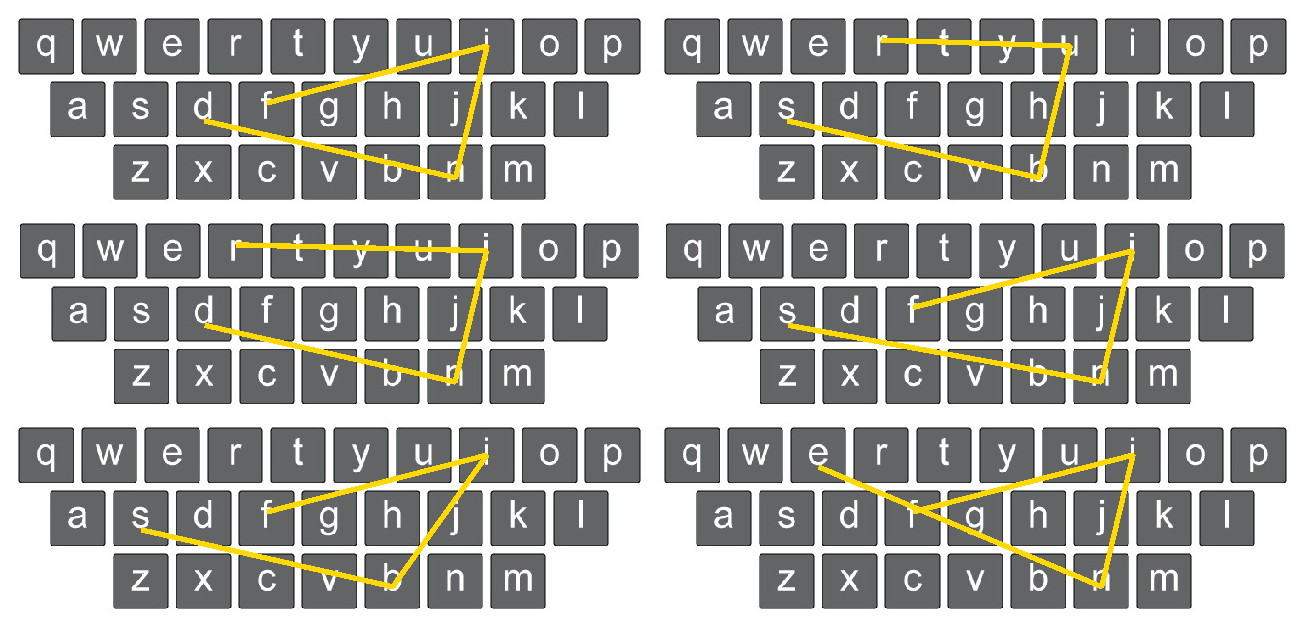
\includegraphics[width=5in]{Figures/fig_words_4}
	\caption[Word Set 4]{The similar gesture-shapes of the word set: `find', `rubs', `rind', `fins', `fibs', `fine'. These gesture-shapes were generated by minimizing dissimilarity using the custom dissimilarity algorithm in Section~\ref{gesture_shape_dissimilarity}.}
	\label{fig_words_4}
\end{figure}

\begin{figure}[b]
	\centering
	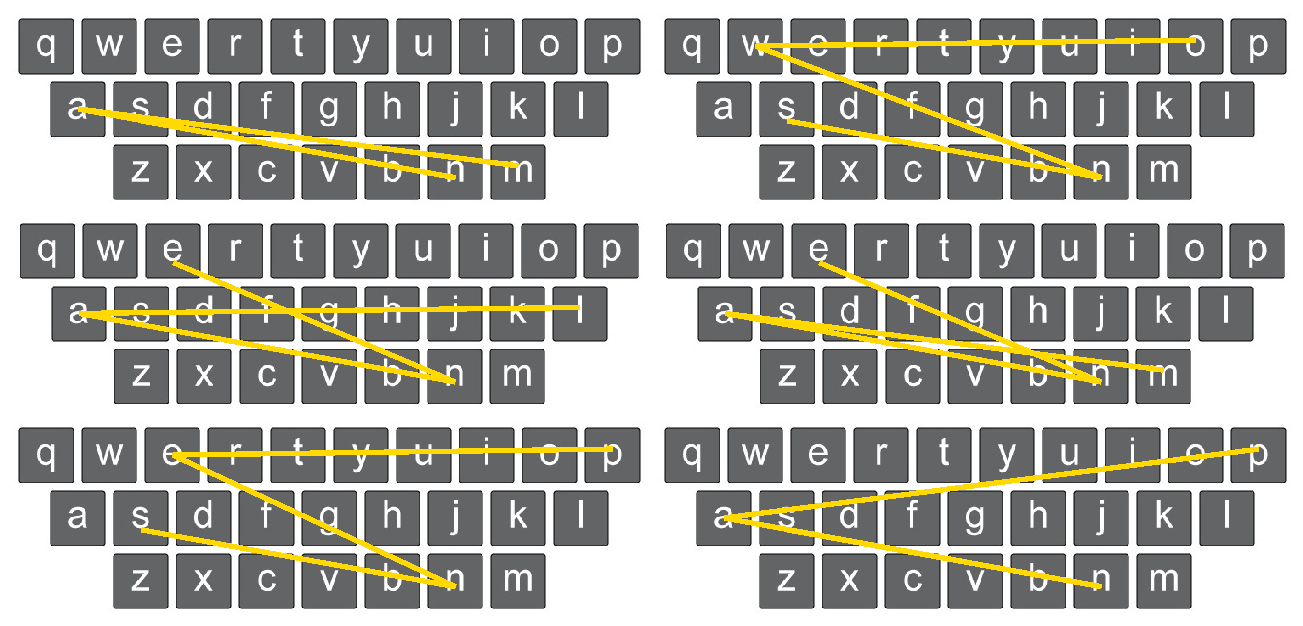
\includegraphics[width=5in]{Figures/fig_words_5}
	\caption[Word Set 5]{The similar gesture-shapes of the word set: `mans', `owns', `lane', `mane', `pens', `pans'. These gesture-shapes were generated by minimizing dissimilarity using the custom dissimilarity algorithm in Section~\ref{gesture_shape_dissimilarity}.}
	\label{fig_words_5}
\end{figure}

\clearpage

\begin{figure}[t]
	\centering
	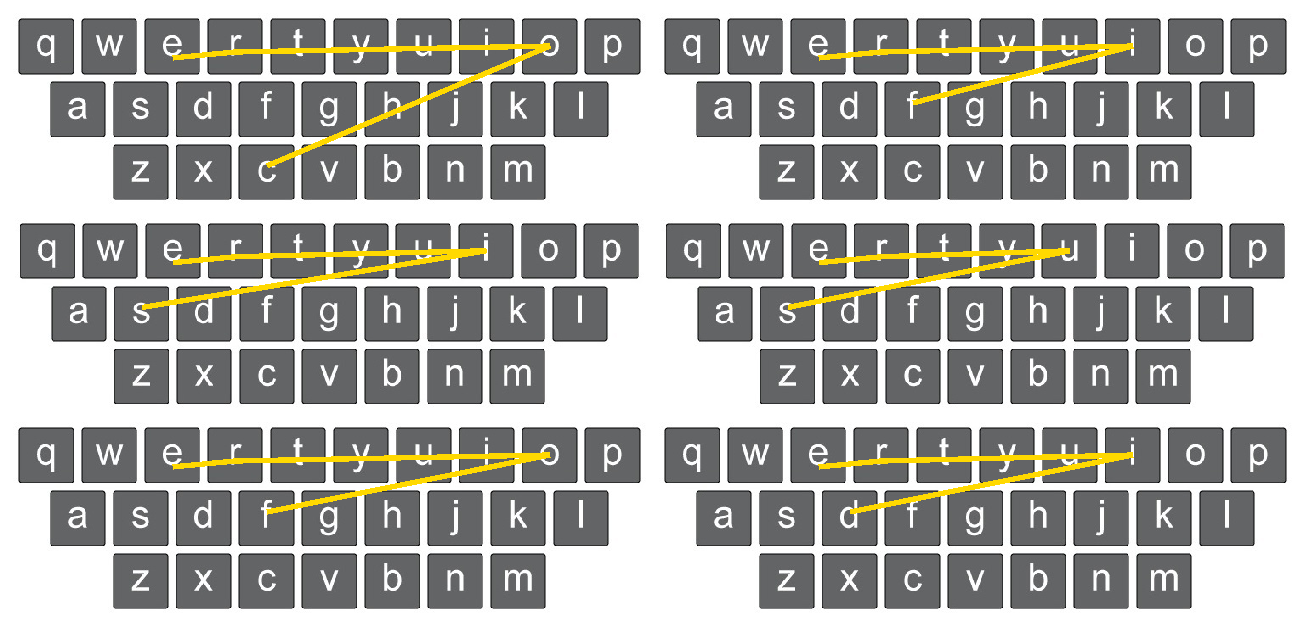
\includegraphics[width=5in]{Figures/fig_words_6}
	\caption[Word Set 6]{The similar gesture-shapes of the word set: `core', `fire', `sire', `sure', `fore', `dire'. These gesture-shapes were generated by minimizing dissimilarity using the custom dissimilarity algorithm in Section~\ref{gesture_shape_dissimilarity}.}
	\label{fig_words_6}
\end{figure}

\begin{figure}[b]
	\centering
	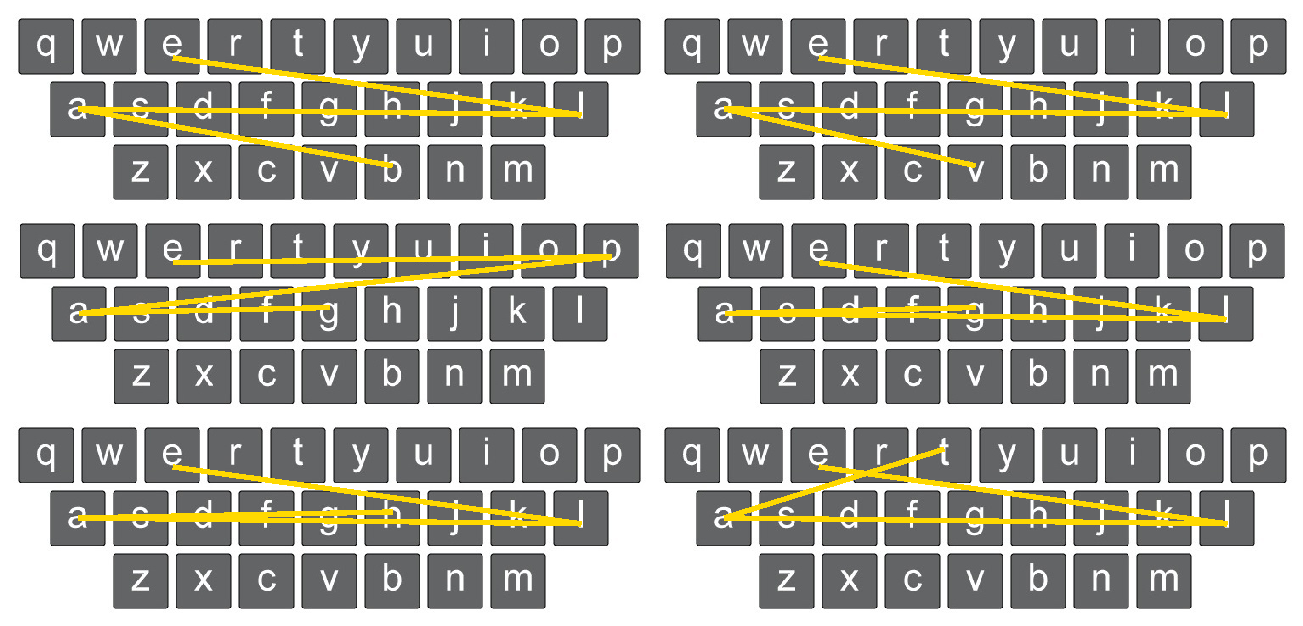
\includegraphics[width=5in]{Figures/fig_words_7}
	\caption[Word Set 7]{The similar gesture-shapes of the word set: `bale', `vale', `gape', `gale', `hale', `tale'. These gesture-shapes were generated by minimizing dissimilarity using the custom dissimilarity algorithm in Section~\ref{gesture_shape_dissimilarity}.}
	\label{fig_words_7}
\end{figure}

\clearpage

\begin{figure}[t]
	\centering
	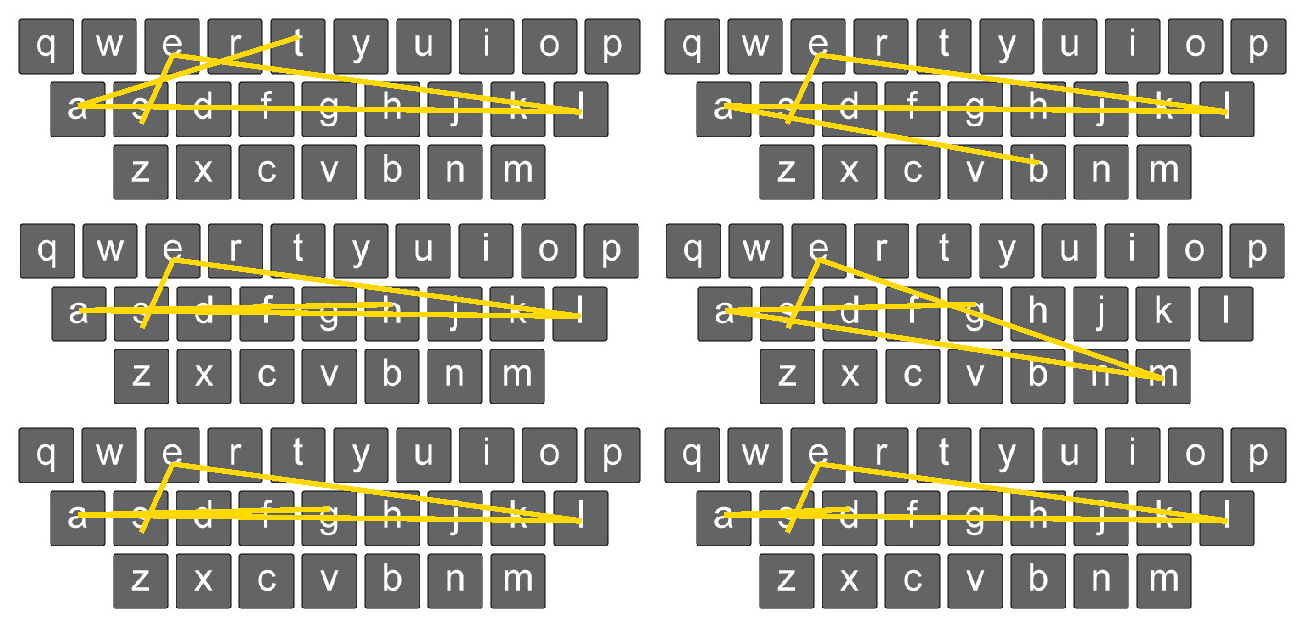
\includegraphics[width=5in]{Figures/fig_words_8}
	\caption[Word Set 8]{The similar gesture-shapes of the word set: `tales', `bales', `hales', `games', `gales', `dales'. These gesture-shapes were generated by minimizing dissimilarity using the custom dissimilarity algorithm in Section~\ref{gesture_shape_dissimilarity}.}
	\label{fig_words_8}
\end{figure}

\begin{figure}[b]
	\centering
	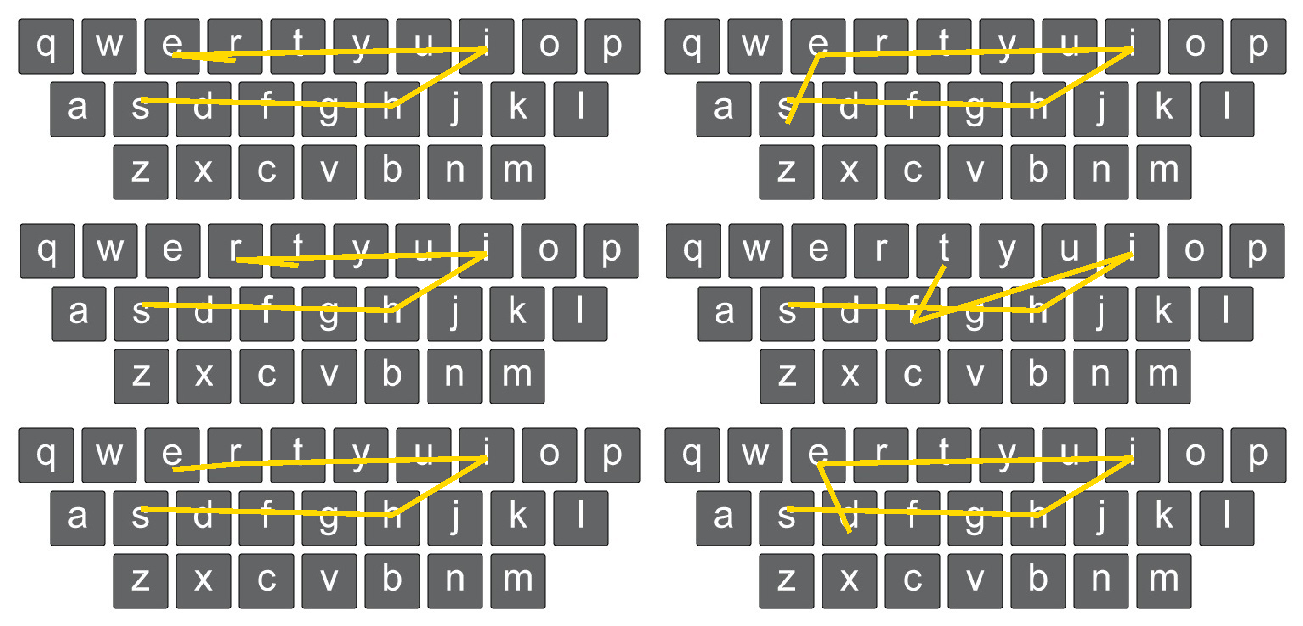
\includegraphics[width=5in]{Figures/fig_words_9}
	\caption[Word Set 9]{The similar gesture-shapes of the word set: `shier', `shies', `shirt', `shift', `shire', `shied'. These gesture-shapes were generated by minimizing dissimilarity using the custom dissimilarity algorithm in Section~\ref{gesture_shape_dissimilarity}.}
	\label{fig_words_9}
\end{figure}

\clearpage

\begin{figure}[t]
	\centering
	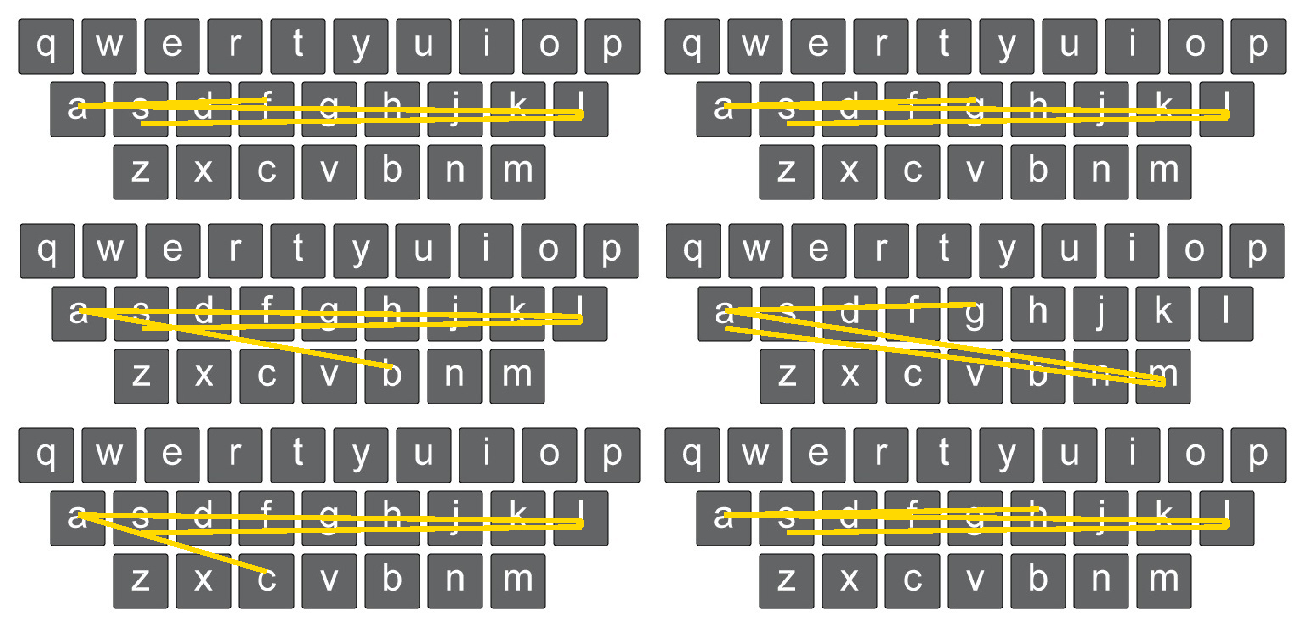
\includegraphics[width=5in]{Figures/fig_words_10}
	\caption[Word Set 10]{The similar gesture-shapes of the word set: `falls', `galls', `balls', `gamma', `calls', `halls'. These gesture-shapes were generated by minimizing dissimilarity using the custom dissimilarity algorithm in Section~\ref{gesture_shape_dissimilarity}.}
	\label{fig_words_10}
\end{figure}

\begin{figure}[b]
	\centering
	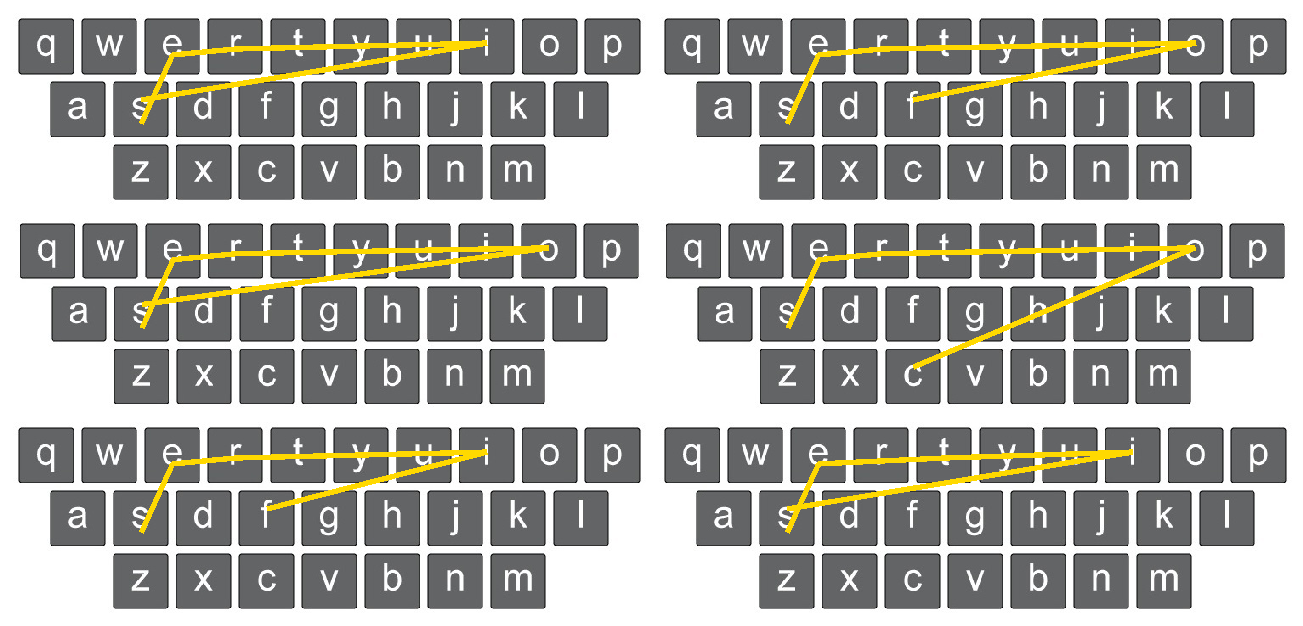
\includegraphics[width=5in]{Figures/fig_words_11}
	\caption[Word Set 11]{The similar gesture-shapes of the word set: `sires', `fores', `sores', `cores', `fires', `sites'. These gesture-shapes were generated by minimizing dissimilarity using the custom dissimilarity algorithm in Section~\ref{gesture_shape_dissimilarity}.}
	\label{fig_words_11}
\end{figure}

\clearpage

\begin{figure}[t]
	\centering
	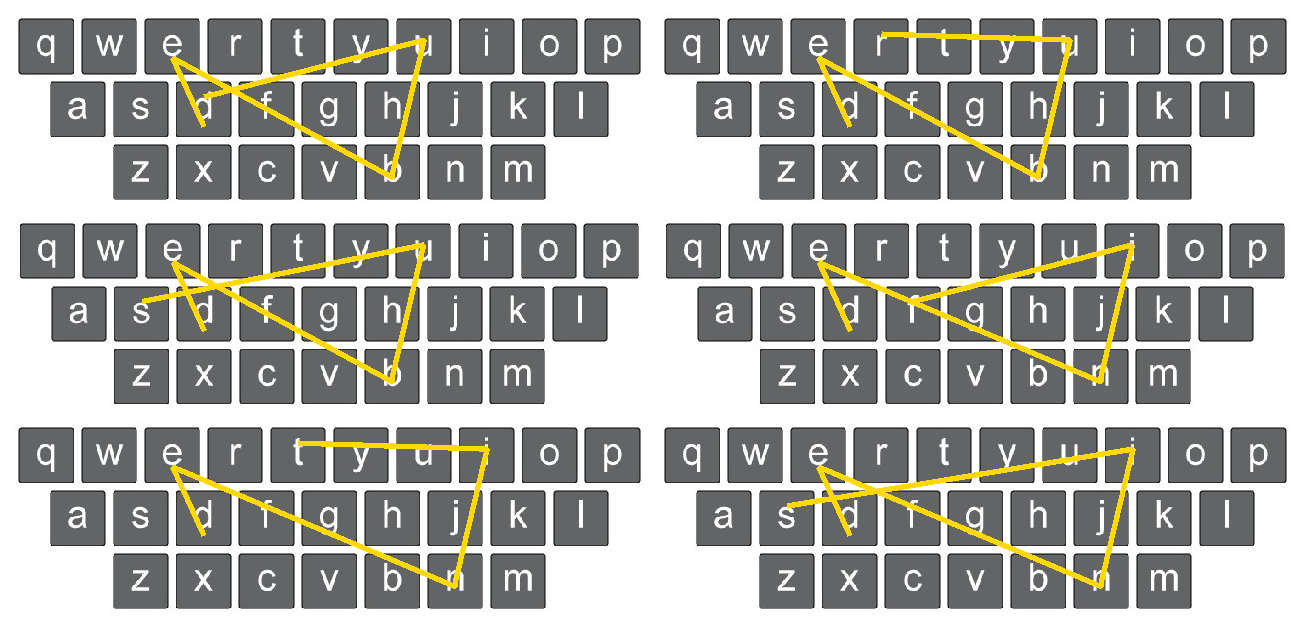
\includegraphics[width=5in]{Figures/fig_words_12}
	\caption[Word Set 12]{The similar gesture-shapes of the word set: `dubbed', `rubbed', `subbed', `finned', `tinned', `sinned'. These gesture-shapes were generated by minimizing dissimilarity using the custom dissimilarity algorithm in Section~\ref{gesture_shape_dissimilarity}.}
	\label{fig_words_12}
\end{figure}

\begin{figure}[b]
	\centering
	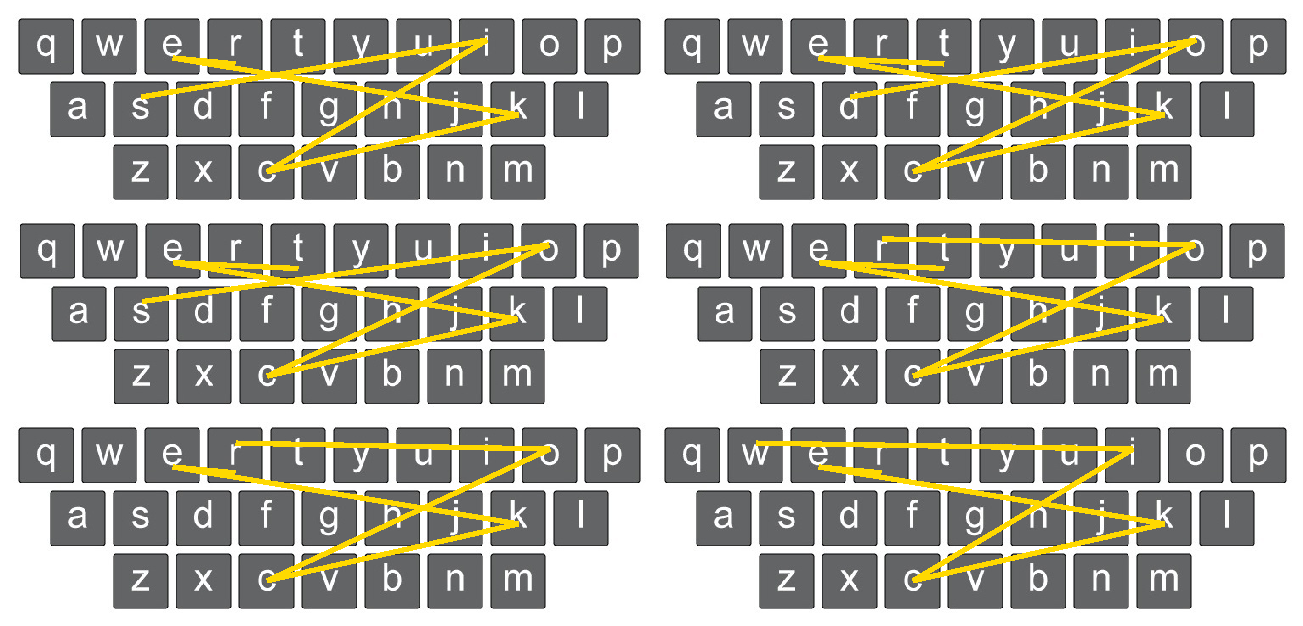
\includegraphics[width=5in]{Figures/fig_words_13}
	\caption[Word Set 13]{The similar gesture-shapes of the word set: `sicker', `docket', `socket', `rocket', `rocker', `wicker'. These gesture-shapes were generated by minimizing dissimilarity using the custom dissimilarity algorithm in Section~\ref{gesture_shape_dissimilarity}.}
	\label{fig_words_13}
\end{figure}

\clearpage

\begin{figure}[t]
	\centering
	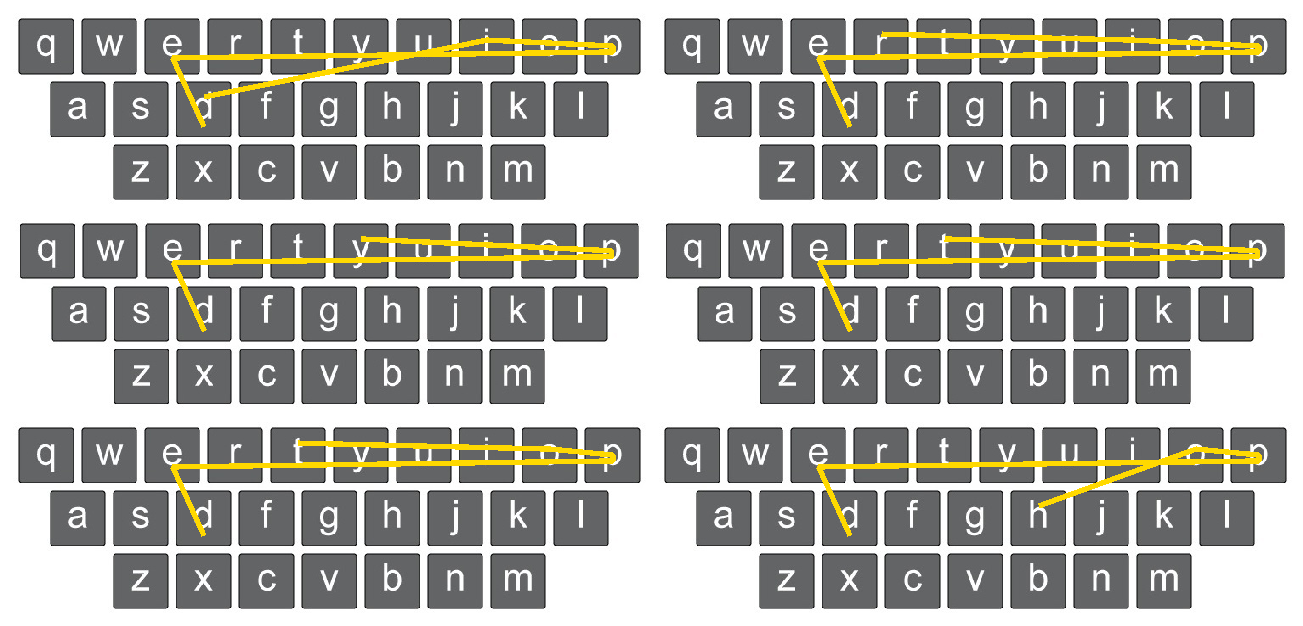
\includegraphics[width=5in]{Figures/fig_words_14}
	\caption[Word Set 14]{The similar gesture-shapes of the word set: `dipped', `ripped', `yipped', `tipped', `topped', `hopped'. These gesture-shapes were generated by minimizing dissimilarity using the custom dissimilarity algorithm in Section~\ref{gesture_shape_dissimilarity}.}
	\label{fig_words_14}
\end{figure}

\begin{figure}[b]
	\centering
	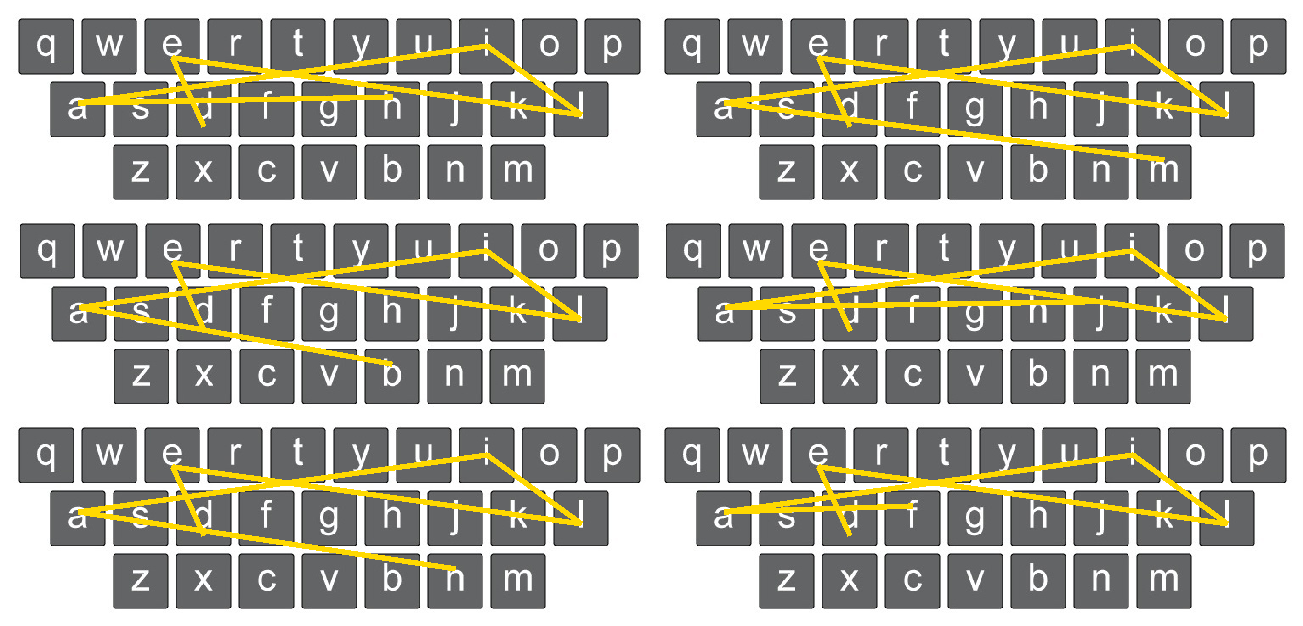
\includegraphics[width=5in]{Figures/fig_words_15}
	\caption[Word Set 15]{The similar gesture-shapes of the word set: `hailed', `mailed', `bailed', `jailed', `nailed', `failed'. These gesture-shapes were generated by minimizing dissimilarity using the custom dissimilarity algorithm in Section~\ref{gesture_shape_dissimilarity}.}
	\label{fig_words_15}
\end{figure}